\documentclass[a4paper]{article}

\usepackage{graphicx}
\usepackage{hyperref}

\pagestyle{empty}

\parindent=0pt
\parskip=1.5em

\setlength{\hoffset}{-1in}
\setlength{\voffset}{-1in}
\setlength{\oddsidemargin}{80mm}
\setlength{\topmargin}{0mm}
\setlength{\headheight}{0mm}
\setlength{\headsep}{0mm}
\setlength{\textheight}{297mm}
\setlength{\textwidth}{50mm}
\setlength{\marginparsep}{0mm}
\setlength{\marginparwidth}{0mm}
\setlength{\footskip}{0mm}

\begin{document}

\vspace*{\fill}

\includegraphics[width=\textwidth]{image/euclid.ps}

\begin{center}
  \Huge
  Euclids\\
  Recipe
\end{center}

Start with two natural number, say 55 and 89.

Repeatedly substract the smaller number from the larger number until
both numbers are equal.

\begin{center}
  \begin{tabular}{cc}
    55 & 89 \\
    55 & 34 \\
    21 & 34 \\
    21 & 13 \\
    8 & 13 \\
    8 &  5 \\
    3 &  5 \\
    3 &  2 \\
    1 &  2 \\
    1 &  1 \\
  \end{tabular}
\end{center}

This number is the greatest common divisor of the numbers you started with.

For an interactive version see\\
{\scriptsize\url{http://dvberkel.github.com/euclids-recipe}}

\vspace{\fill}

\end{document}
